\chapter{ПРОЕКТИРОВАНИЕ И РЕАЛИЗАЦИЯ АРХИТЕКТУРЫ ВЕБ-ПРИЛОЖЕНИЯ}

\section{Анализ структуры исходных данных}
Для корректной обработки информации маркетплейсов исследованы форматы и структура ключевых отчётов, получаемых с помощью API: отчёт о продажах (CSV) и отчёт об остатках по кластерам (XLSX). Данные форматы являются стандартизированными и машинно-читаемыми, что позволяет автоматизировать их обработку.

\subsection{Отчет о продажах (CSV)}
Отчёт содержит транзакционные данные, где каждая строка соответствует товарной позиции в заказе. Названия столбцов для анализа отчета: 

\begin{enumerate}
\item Принят в обработку – дата оформления заказа;
\item Статус – статус заказа («Доставлен»/«Отменен»/«Доставляется»);
\item Сумма отправления – стоимость заказа;
\item Название товара – наименование товара на маркетплейсе;
\item Количество – количество товаров в одном заказе.
\end{enumerate}

\subsection{Отчёт об остатках по кластерам (XLSX)}
Отчёт отражает распределение товарных запасов по складам (кластерам) маркетплейса. Ключевые поля:

\begin{enumerate}
\item Название товара – наименование товара на маркетплейсе;
\item Кластер – Город размещения склада;
\item Ликвидность – на сколько интересным товар в кластере;
\item Среднесуточные продажи – среднее арифметическое всех продаж;
\item Остатки на складах – количество остатков товара в кластере.
\end{enumerate}

Помимо вышесказанного, требуется произвести нормализацию данных для обеспечения устойчивости к изменениям формата отчетов. Алгоритм реализован по методу адаптивного парсинга, который идентифицирует колонки по их содержанию (например, поиск подстроки «Количество»). 

Таким образом, структура исходных отчётов содержит все необходимые данные для реализации трёх модулей аналитики: расчёта юнит-экономики, анализа динамики продаж и прогнозирования остатков на кластерах.

\section{Адаптивный парсинг и валидация данных}

Исходные отчёты маркетплейсов (CSV и XLSX) не имеют жёстко фиксированной структуры: маркетплейсы могут изменять порядок столбцов, добавлять новые поля или переименовывать существующие. Прямая привязка к индексам столбцов привела бы к частым ошибкам при обновлении форматов выгрузки. Для решения этой проблемы реализован адаптивный парсинг – метод, при котором система автоматически идентифицирует необходимые столбцы, по ключевым словам, в заголовках, независимо от их позиции в файле.

\subsection{Адаптивный парсинг веб – сайта}

На рисунке 2.1 представлена блок-схема алгоритма адаптивного парсинга применительно к отчёту о продажах. Алгоритм выполняет следующие действия:

\begin{enumerate}
\item Проверка файла – если файл пуст или не содержит заголовков, обработка прерывается с сообщением об ошибке;
\item Парсинг заголовков – считываются названия всех столбцов;
\item Поиск целевых колонок – для каждого аналитического поля (дата, название товара, количество, статус, сумма) выполняется поиск подстроки в заголовках. Поиск регистронезависимый названий, допускаются варианты количество, кол-во, quantity;
\item Фиксация индексов – найденные индексы столбцов запоминаются;
\item Заполнение данных – построчный обход файла, извлечение значений по зафиксированным индексам и преобразование типов (даты, числа);
\end{enumerate}

Если какой-либо обязательный столбец не найден, алгоритм возвращает ошибку с указанием отсутствующего поля. Алгоритм парсинга показан на рисунке 2.1.

\begin{figure}[h]
    \centering
    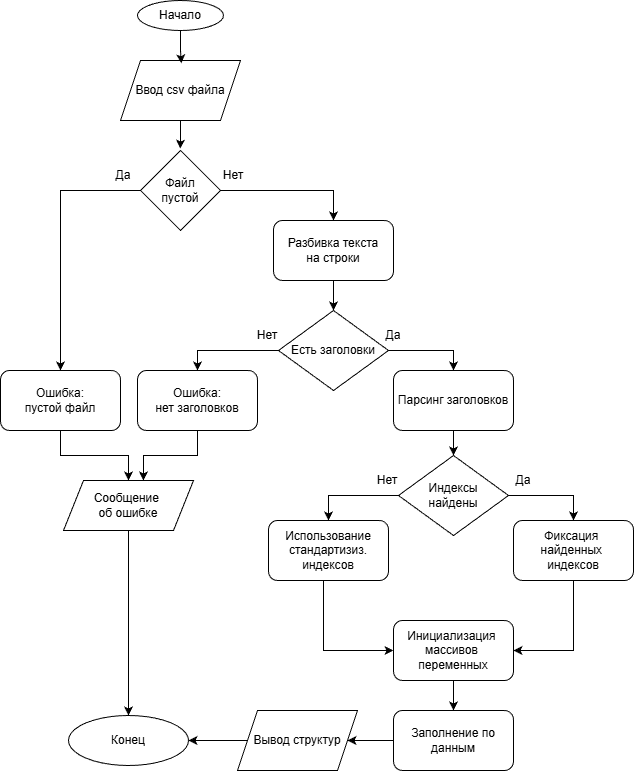
\includegraphics[width=0.9\textwidth]{../image/screen2.png}
    \caption{Пример парсинга файла и валидации данных.}
    \label{fig:example01}
\end{figure}

\subsection{Валидация и обработка ошибок}
После извлечения данных выполняется валидация:
\begin{itemize}
\item проверка формата дат;
\item приведение числовых полей к типу number;
\item фильтрация строк по статусу заказа (только доставленные заказы участвуют в аналитике);
\item отбрасывание строк с некорректными или пустыми значениями.
\end{itemize}

Для XLSX-файлов (отчёт об остатках) алгоритм дополняется выбором активного листа и поиском специфических полей: Кластер, Ликвидность, Среднесуточные продажи, Остатки на складах, Дней без остатка.

При возникновении любой ошибки пользователь получает информативное сообщение на русском языке с указанием причины. Это позволяет быстро исправить проблему без анализа технических логов.

\section{Кластерный анализ }

На основе отчёта об остатках по кластерам (XLSX) разработан модуль кластерного анализа, который позволяет оценить распределение товарных запасов по складам маркетплейса, выявить неликвидные остатки и сформировать рекомендации по пополнению.

\subsection{Исходные данные для анализа}

Модуль использует следующие поля отчёта (см. рис. 2.2.):

\begin{itemize}
\item Товар – id, наименование/артикул товара;
\item Кластер – id, город/название кластера;
\item Остаток товара в кластере – id, товар\_id, кластер\_id, остаток, среднесуточные продажи за 28 дней, ликвидность, дата выгрузки;
\item Прогноз по товару – товар\_id, суммарный остаток, суммарные продажи, дней до исчерпания, рекомендация;
\item Прогноз по кластеру – id, товар\_id, кластер\_id, дней до исчерпания, рекомендация, цветовая зона.
\end{itemize}

Связи между сущностями:

\begin{enumerate}
\item Товар (1) – (М) Остаток товара в кластере. Один товар может храниться во многих кластерах (складах);
\item Кластер (1) – (М) Остаток товара в кластере. В одном кластере может храниться много товаров;
\item Остаток товара в кластере (1) – (1) Прогноз по кластеру. Каждая запись остатка порождает один прогноз для конкретного кластера;
\item Товар (1) – (1) Прогноз по товару. Каждый товар имеет один итоговый прогноз (агрегированный по всем кластерам).
\end{enumerate}



\begin{figure}[h]
    \centering
    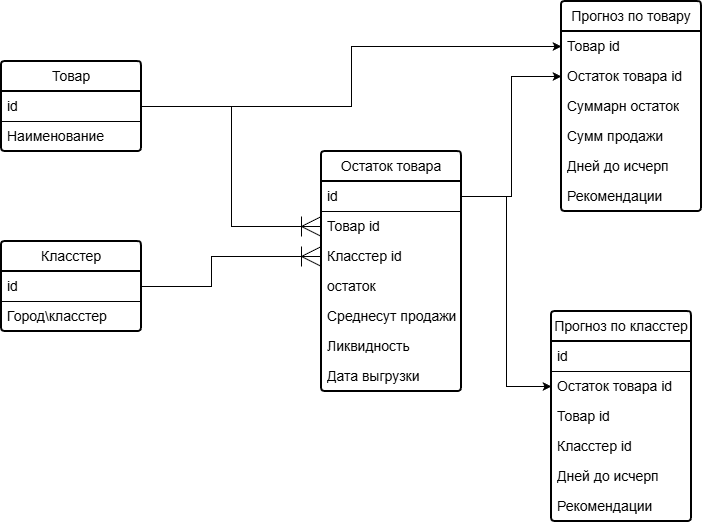
\includegraphics[width=1\textwidth]{../image/er диаграмма класстерного анализа.drawio.png}
    \caption{ER-диаграмма взаимосвязей.}
    \label{fig:example01}
\end{figure}

\subsection{Алгоритм кластерного анализа}

Вычисления выполняются в следующем порядке:

\begin{enumerate}
\item Расчёт уровня локализации товара:

Уровень локализации показывает, в скольких кластерах из всех возможных товар уже представлен:

\begin{equation}
\text{Уровень локализации} = \frac{\text{Количество кластеров с остатком} > 0}{\text{Общее количество кластеров}} \times 100\%
\end{equation}

Чем выше уровень, тем шире географическое присутствие товара. Низкий уровень ($<30\%$) указывает на потенциал расширения.

\item Прогноз остатков (дней до исчерпания):

Для каждого кластера, где товар присутствует, вычисляется, на сколько дней хватит текущего запаса при текущих среднесуточных продажах:

\begin{equation}
\text{Дней до исчерпания} = \frac{\text{Остаток на складе}}{\text{Среднесуточные продажи}}
\end{equation}

Если знаменатель равен нулю (продаж нет), прогноз считается бесконечным – товар не продаётся.

\item Классификация зон пополнения:

На основе прогноза кластеры разделяются на три зоны:

\begin{itemize}
\item красная зона (дней $<30$) – требуется срочное пополнение;
\item жёлтая зона ($30$–$60$ дней) – плановое пополнение в ближайшее время;
\item зелёная зона ($>60$ дней) – пополнение не требуется.
\end{itemize}

\item Оценка ликвидности:

Ликвидность определяется на основе переданного показателя из отчёта, и классифицируются по формуле (2.3):

\begin{equation}
\text{Ликвидность} = 
\begin{cases}
\text{Высокая}, & \text{среднесуточные продажи} > 50; \\[4pt]
\text{Средняя}, & \text{если } 10 \leq \text{продажи} \leq 50; \\[4pt]
\text{Низкая}, & \text{если продажи} < 10.
\end{cases}
\end{equation}

Товары с низкой ликвидностью и большими остатками маркируются как «замороженный запас» – рекомендуется уценка или перемещение в более востребованные кластеры.

\item Формирование рекомендаций:

На выходе модуль формирует:

\begin{itemize}
\item Сводную таблицу по каждому товару: кластеры, остатки, прогноз дней, зона пополнения;
\item Список кластеров, требующих срочной поставки;
\item Перечень неликвидных остатков с предложениями по оптимизации.
\end{itemize}

\end{enumerate}

\subsection{Практическая ценность}

Разработанный алгоритм позволяет продавцу автоматически получать ответы на ключевые вопросы:

\begin{itemize}
\item В какие кластеры нужно поставить товар и в каком объёме;
\item В каких кластерах слабая оборачиваемость;
\item Насколько равномерно товар распределён по регионам.
\end{itemize}

Это сокращает время на анализ остатков с нескольких часов до нескольких минут и минимизирует риск упущенных продаж из-за отсутствия товара в востребованных кластерах.

\section{Реализация API}

\subsection{Общая методология работы с API}

Работа с любым современным REST API, например Ozon Seller API, строится на нескольких фундаментальных принципах, которые необходимо учитывать при разработке приложений [8].

Архитектура клиент-серверного взаимодействия, для примера возьмем OZON API, организовано по классической модели запрос-ответ. Клиентское приложение инициирует соединение, отправляя HTTP-запросы на серверы Ozon. Сервер обрабатывает запрос и возвращает ответ в формате JSON. Все запросы выполняются по защищенному протоколу HTTPS, что гарантирует шифрование передаваемых данных и защиту от перехвата конфиденциальной информации.

Ключевым требованием для работы с API является наличие действующих учетных данных продавца. Для работы потребуется client id и API токен, при каждом запросе к API эти данные передаются в HTTP-заголовках, что обеспечивает идентификацию отправителя и проверку его прав доступа.

Особенностью работы с отчетами в Ozon API является асинхронная модель обработки запросов. При запросе большого объема данных сервер не возвращает их мгновенно, а создает задачу на формирование отчета и предоставляет уникальный идентификатор (code), по которому впоследствии можно получить готовый отчет. Такой подход позволяет эффективно распределять серверные ресурсы и обрабатывать запросы любого объема без риска превышения таймаутов соединения.

Для получения отчетов по API требуется использования трех ключевых методов Ozon Seller API, которые в совокупности реализуют полный цикл получения отчетов по отправлениям [8].

\subsection{Метод создания отчета: POST /v1/report/postings/create}

Данный метод инициирует процесс формирования отчета по отправлениям за указанный временной период [8].

В теле запроса клиент передает фильтр с параметрами выборки:

\begin{code}
\captionof{listing}{Фильтры с параметрами выборки для интеграции API Ozon seller c веб приложением}
\label{code:openmp}
\vspace{-0.75cm}\begin{minted}[mathescape,linenos,frame=lines,breaklines]{C}
const requestBody = {
    filter: {
        processed_at_from: formatDate(fromDate),
        processed_at_to: formatDate(toDate),
        delivery_schema: [deliverySchema],
        statuses: []
    },
    language: 'DEFAULT'
};
\end{minted}
\end{code}

Критически важным требованием спецификации является передача параметра delivery schema в виде массива, даже если указывается только одно значение (например, ["fbo"] или ["fbs"]). В случае успешного создания задачи сервер возвращает объект с уникальным кодом отчета. Этот код сохраняется в приложении и используется для последующей проверки статуса готовности [8].

\subsection{Метод проверки статуса: POST /v1/report/info}

Поскольку формирование отчета может занимать от нескольких секунд до нескольких минут (в зависимости от объема данных и загрузки серверов), необходим механизм проверки готовности результата. Метод info принимает код отчета и возвращает актуальную информацию о его состоянии [8].

\begin{code}
\captionof{listing}{Реализация цикла опроса сервера для получения отчета с экспоненциальной задержкой}
\label{code:openmp}
\vspace{-0.75cm}\begin{minted}[mathescape,linenos,frame=lines,breaklines]{C}
for (let i = 0; i < 30; i++) {
    const response = await fetch('https://api-seller.ozon.ru/v1/report/info', {
        method: 'POST',
        headers: { ... },
        body: JSON.stringify({ code })
    });

    const data = await response.json();
    if (data.result.status === 'success') {
        return data.result;
    }
    await sleep(2000);
}
\end{minted}
\end{code}

В процессе работы метод может возвращать следующие статусы [8]:

\begin{itemize}
\item pending / waiting / processing — отчет еще формируется, необходимо повторить запрос позже;
\item success — отчет готов к скачиванию, в ответе присутствует прямая ссылка на файл;
\item error — при формировании отчета произошла ошибка (например, указан некорректный период).
\end{itemize}

При успешной готовности метод возвращает объект, содержащий ссылку для скачивания сформированного файла.

\subsection{Получение отчета }

Заключительный этап — получение файла отчета по предоставленной ссылке. В отличие от предыдущих методов, этот запрос не требует специальных заголовков авторизации, так как ссылка является временной и одноразовой.

В процессе разработки было установлено, что файлы отчетов могут передаваться в различных форматах (CSV, XLSX) и кодировках. Наиболее надежный подход — сохранять файл в бинарном виде, полностью сохраняя исходное форматирование:

\begin{code}
\captionof{listing}{Реализация цикла опроса сервера для получения отчета с экспоненциальной задержкой}
\label{code:openmp}
\vspace{-0.75cm}\begin{minted}[mathescape,linenos,frame=lines,breaklines]{C}
const response = await fetch(fileUrl, {
    agent: new https.Agent({ keepAlive: true })
});

const buffer = await response.buffer();
fs.writeFileSync(filePath, buffer);

\end{minted}
\end{code}

В некоторых случаях Ozon возвращает файлы в кодировке Windows-1251, что при открытии в современных редакторах приводит к отображению нечитаемых символов. Для решения этой проблемы в приложении реализована автоматическая конвертация.

\begin{code}
\captionof{listing}{Реализация цикла опроса сервера для получения отчета с экспоненциальной задержкой}
\label{code:openmp}
\vspace{-0.75cm}\begin{minted}[mathescape,linenos,frame=lines,breaklines]{C}
try {
    content = buffer.toString('utf8');
} catch {
    content = iconv.decode(buffer, 'win1251');
}
\end{minted}
\end{code}

\section{Модульная структура веб API системы}

Приложение построено по модульному принципу, где каждая функция отвечает за отдельный этап взаимодействия с API [8]:

\begin{table}[H]
\caption{Функции для работы с отчетами Ozon API}
\label{tab:report-functions}
\begin{tabular}{|l|l|l|l|}
\hline
Функция & Назначения & Входные параметры & Возвращаемое значение \\ \hline
createReport & Создание отчета & Параметры фильтрации & Код отчета \\ \hline
waitForReport & Проверка статуса & Код отчета & Информация с ссылкой \\ \hline
downloadReport & Скачивание файла & URL, тип отчета & Путь к сохраненному файлу \\ \hline
\end{tabular}
\end{table}

\section{Обработка ошибок и исключений}
Все запросы к API обернуты в блоки try/catch для корректной обработки возможных сбоев:

\begin{itemize}
\item Ошибки сети — таймауты, разрывы соединения;
\item Ошибки авторизации — неверный Client ID или API-ключ;
\item Ошибки валидации — некорректные параметры запроса;
\item Ошибки сервера — временные проблемы на стороне Ozon.
\end{itemize}

\begin{code}
\captionof{listing}{Обработка сбоев}
\label{code:openmp}
\vspace{-0.75cm}\begin{minted}[mathescape,linenos,frame=lines,breaklines]{C}
try {
    const response = await fetch(url, options);
    const data = await response.json();
    
    if (!response.ok) {
        throw new Error(`Ошибка API: ${JSON.stringify(data)}`);
    }
    
    return data.result;
} catch (error) {
    log(` Ошибка: ${error.message}`, 'ERROR');
    throw error;
}

\end{minted}
\end{code}

\section{Анализ структуры входных данных}
Для корректной обработки информации маркетплейсов исследованы форматы и структура ключевых отчётов: отчёт о продажах (CSV) и отчёт об остатках по кластерам (XLSX). Данные форматы являются стандартизированными и машинно-читаемыми, что позволяет автоматизировать их обработку.

\subsection{Отчет о продажах (CSV) }

Отчёт содержит транзакционные данные, где каждая строка соответствует товарной позиции в заказе. Названия столбцов для анализа отчета:

\begin{enumerate}
\item Принят в обработку – дата оформления заказа;
\item Статус – статус заказа («Доставлен»/«Отменен»/«Доставляется»);
\item Сумма отправления – стоимость заказа;
\item Название товара – наименование товара на маркетплейсе;
\item Количество – количество товаров в одном заказе.
\end{enumerate}

\subsection{Отчёт об остатках по кластерам (XLSX)}

Отчёт отражает распределение товарных запасов по складам (кластерам) маркетплейса. Ключевые поля:

\begin{enumerate}
\item Название товара – наименование товара на маркетплейсе;
\item Кластер – Город размещения склада;
\item Ликвидность – на сколько интересным товар в кластере;
\item Среднесуточные продажи – среднее арифметическое всех продаж;
\item Остатки на складах – количество остатков товара в кластере.
\end{enumerate}

Помимо вышесказанного, требуется произвести нормализацию данных для обеспечения устойчивости к изменениям формата отчетов. Алгоритм реализован по методу адаптивного парсинга, который идентифицирует колонки по их содержанию (например, поиск подстроки «Количество»).

Таким образом, структура исходных отчётов содержит все необходимые данные для реализации трёх модулей аналитики: расчёта юнит-экономики, анализа динамики продаж и прогнозирования остатков на кластерах.

\section{Проектирование системы обработки данных}
Архитектура системы построена на принципах клиент-серверной модели с обработкой на стороне клиента. Основная цель архитектуры – преобразование сырых данных из форматов CSV/XLSX в структурированные аналитические показатели через последовательные обработки.

Блок-схема процесса обработки данных представлена на рисунке 2.1

\begin{figure}[h]
    \centering
    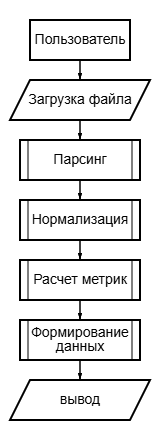
\includegraphics[width=0.2\textwidth]{../image/screen3.png}
    \caption{Архитектура обработки данных.}
    \label{fig:example02}
\end{figure}

\subsection{Алгоритм парсинга и нормализации данных}

Алгоритм парсинга получаемых API CSV-отчетов (данные о продажах) предназначен для преобразования текстовых CSV-файлов в структурированные данные. Процесс состоит из следующих шагов:

\begin{enumerate}
\item Получение разрешения на доступ к API отчетам;
\item Запрос на получение API отчета;
\item Получение API отчета;
\item Чтение файла – получение CSV как текстовой строки;
\item Разделение на строки – разбиение текста по символам новой строки;
\item Определение структуры:
\begin{itemize}
\item Первая строка обрабатывается как заголовок;
\item Определяются индексы нужных колонок по их названиям;
\item Если колонка не найдена по названию, используется стандартный индекс.
\end{itemize}
\item Обработка данных – для каждой строки:
\begin{itemize}
\item Извлечение значений по определенным индексам;
\item Парсинг дат с учетом разных форматов;
\item Классификация заказов по статусам.
\end{itemize}
\end{enumerate}

Алгоритм парсинга XLSX-отчетов (данные об остатках по кластерам) предназначен для обработки Excel-файлов с информацией о распределении товаров по складам:

\begin{enumerate}
\item Чтение файла – получение XLSX файла;
\item Поиск нужного листа – идентификация рабочего листа с данными;
\item Определение начала данных – пропуск заголовочных строк (первые 4 строки);
\item Извлечение данных – чтение значений из конкретных колонок:
\begin{itemize}
\item Колонка F – название кластера (склада);
\item Колонка B – название товара;
\item Колонка K – количество остатков;
\item Колонка L – товары в процессе подготовки;
\item Колонка O – товары с истекающим сроком;
\item Колонка V – возвращаемые товары.
\end{itemize}
\item Фильтрация – удаление служебных и пустых строк;
\item Структурирование – преобразование в табличную форму (товары + кластеры);
\end{enumerate}

\subsection{Алгоритм валидации данных}

Процесс проверки корректности вводимых и обрабатываемых данных:

\begin{enumerate}
\item Проверка типов данных – соответствие ожидаемым типам;
\item Валидация числовых значений:
\begin{itemize}
\item Проверка на числовой тип;
\item Проверка на отрицательные значения;
\item Обработка некорректных значений (замена на 0).
\end{itemize}
\item Проверка форматов:
\begin{itemize}
\item Валидация форматов дат;
\item Проверка текстовых полей на наличие данных.
\end{itemize}
\item Визуальная индикация – выделение полей с ошибками;
\end{enumerate}

Данная архитектура обеспечивает надежную обработку данных без необходимости в серверной инфраструктуре, что соответствует требованиям доступности и безопасности системы.

\section{Авторизация пользователей}

Для разграничения доступа к аналитическим данным в веб-приложении реализована подсистема аутентификации и авторизации. Она обеспечивает регистрацию новых пользователей, вход зарегистрированных пользователей, защиту маршрутов от несанкционированного доступа и безопасное хранение учётных данных. Система построена на следующих компонентах.

\subsection{Регистрация и вход пользователей}

Регистрация нового пользователя выполняется по паре «email – пароль». При регистрации пользователь указывает свой email и пароль (минимальная длина — 6 символов). Сервер проверяет уникальность email — если пользователь с таким адресом уже существует, возвращается ошибка. Пароль никогда не хранится в открытом виде, а подвергается хешированию с помощью библиотеки bcrypt. При входе пользователь вводит email и пароль, сервер находит запись в базе данных, сравнивает хеш введённого пароля с сохранённым и при совпадении открывает доступ.

\begin{code}
\captionof{listing}{Хеширование пароля при регистрации}
\label{code:openmp}
\vspace{-0.75cm}\begin{minted}[mathescape,linenos,frame=lines,breaklines]{C}
const salt = await bcrypt.genSalt(10);
const passwordHash = await bcrypt.hash(password, salt);
\end{minted}
\end{code}

\begin{code}
\captionof{listing}{Сравнение пароля при входе}
\label{code:openmp}
\vspace{-0.75cm}\begin{minted}[mathescape,linenos,frame=lines,breaklines]{C}
const isValid = await bcrypt.compare(password, user.password_hash);
\end{minted}
\end{code}

\subsection{Управление сессией с помощью JWT-токенов}

После успешной аутентификации сервер генерирует JWT-токен (JSON Web Token), который содержит идентификатор пользователя и его email. Токен подписывается секретным ключом, хранящимся в переменных окружения, и имеет ограниченное время жизни (7 дней). Это позволяет автоматически завершать сессию по истечении срока без необходимости хранить состояние на сервере.

\begin{code}
\captionof{listing}{Создание JWT-токена}
\label{code:openmp}
\vspace{-0.75cm}\begin{minted}[mathescape,linenos,frame=lines,breaklines]{C}
const payload = { userId: user.id, email: user.email };
const token = jwt.sign(payload, process.env.JWT_SECRET, { expiresIn: '7d' });
\end{minted}
\end{code}

\subsection{Безопасное хранение токена}

Сгенерированный JWT-токен устанавливается в HTTP-only cookie. Флаг httpOnly запрещает доступ к cookie из клиентского JavaScript-кода, что эффективно защищает токен от XSS-атак. Дополнительно устанавливаются флаги sameSite=lax (защита от CSRF) и secure в production-среде (передача только по HTTPS). При каждом последующем запросе браузер автоматически отправляет эту cookie на сервер.



\begin{code}
\captionof{listing}{Установка HTTP-only cookie}
\label{code:openmp}
\vspace{-0.75cm}\begin{minted}[mathescape,linenos,frame=lines,breaklines]{C}
response.cookies.set({
  name: 'session',
  value: token,
  httpOnly: true,
  path: '/',
  maxAge: 60 * 60 * 24 * 7,
  sameSite: 'lax',
});
\end{minted}
\end{code}

\subsection{Защита маршрутов (middleware/proxy)}
Для предотвращения доступа неавторизованных пользователей к защищённым разделам приложения (страницы аналитики, дашборд) реализован middleware-компонент (в Next.js версии 16 называется proxy.ts). Функция выполняется на сервере перед обработкой каждого входящего запроса, проверяет наличие и валидность JWT-токена в cookie и принимает решение:

Если пользователь не авторизован и пытается зайти на защищённую страницу – происходит перенаправление на страницу входа (/login);

Если пользователь авторизован и пытается зайти на страницу входа или регистрации – перенаправление на главную страницу (/);

Если пользователь авторизован и запрашивает разрешённую страницу – запрос пропускается.



\begin{code}
\captionof{listing}{Пример middleware-проверки}
\label{code:openmp}
\vspace{-0.75cm}\begin{minted}[mathescape,linenos,frame=lines,breaklines]{C}
const token = request.cookies.get('session')?.value;
const isAuthenticated = token ? verifySessionToken(token) !== null : false;

if (!isAuthenticated && !isPublicPath) {
  return NextResponse.redirect(new URL('/login', request.url));
}
\end{minted}
\end{code}

\subsection{База данных пользователей}
Для постоянного хранения учётных записей используется реляционная база данных. Таблица users содержит следующие поля:

\begin{table}[H]
\caption{Структура таблицы пользователей}
\label{tab:users}
\begin{tabular}{|l|l|l|}
\hline
\textbf{Поле} & \textbf{Тип} & \textbf{Описание} \\ \hline
id & TEXT (PRIMARY KEY) & Уникальный идентификатор пользователя (UUID) \\ \hline
email & TEXT (UNIQUE) & Адрес электронной почты (используется как логин) \\ \hline
password\_hash & TEXT & Хеш пароля, сгенерированный bcrypt \\ \hline
created\_at & DATETIME & Дата и время регистрации \\ \hline
\end{tabular}
\end{table}

\subsection{Выход из системы}
При нажатии кнопки «Выйти» клиент отправляет запрос на сервер, который удаляет cookie с токеном сессии. После этого пользователь перенаправляется на страницу входа.

\begin{code}
\captionof{listing}{Выход из системы}
\label{code:openmp}
\vspace{-0.75cm}\begin{minted}[mathescape,linenos,frame=lines,breaklines]{C}
response.cookies.delete('session');
return NextResponse.redirect(new URL('/login', request.url));
\end{minted}
\end{code}

\subsection{Схема работы авторизации}

На рисунке 2.4 представлена общая схема работы подсистемы авторизации:

Пользователь регистрируется → пароль хешируется → сохраняется в БД;

Пользователь входит → сервер проверяет пароль → генерирует JWT → устанавливает HTTP-only cookie;

При переходе на любую страницу middleware проверяет валидность cookie;

При выходе cookie удаляется.

Таким образом, реализованная подсистема обеспечивает надёжную защиту пользовательских данных, удобство использования и масштабируемость. Все пароли хранятся в хешированном виде, токены сессий защищены от XSS-атак, а маршруты централизованно контролируются через middleware.

\begin{figure}[pt]
    \centering
    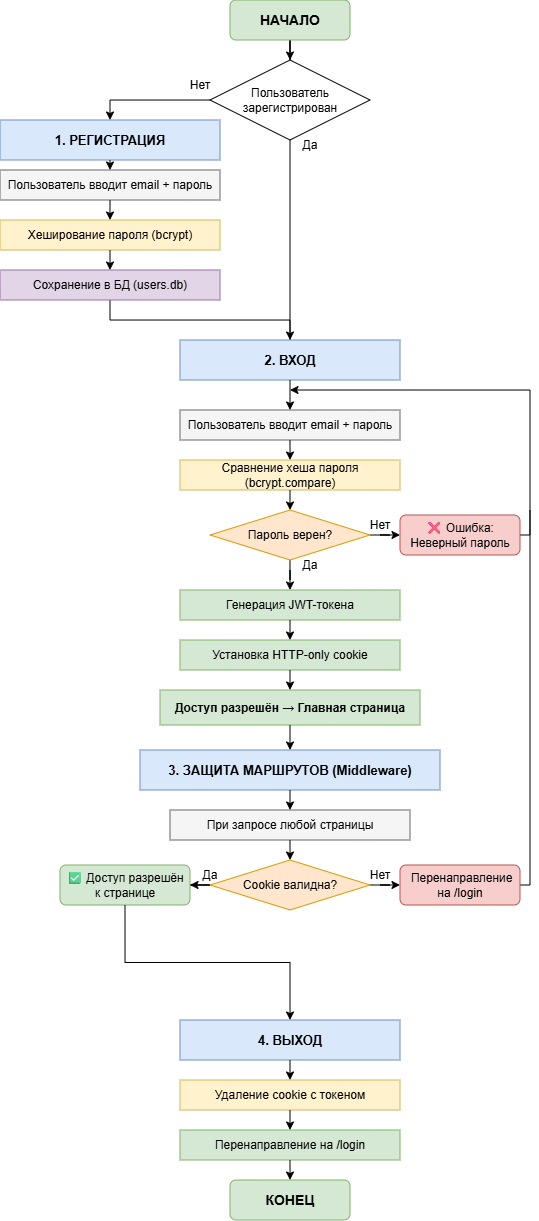
\includegraphics[width=0.7\textwidth]{../image/screen4.png}
    \caption{Схема работы системы авторизации.}
    \label{fig:example02}
\end{figure}